\documentclass[12pt]{article}
\usepackage[svgnames,x11names,table]{xcolor}
\usepackage{hyperref}
\usepackage{graphicx}
\usepackage{parskip}
\usepackage{float}
\usepackage{amsmath}
\usepackage{amssymb}
\usepackage{enumitem}
\usepackage[thicklines]{cancel}

\hypersetup{
    colorlinks,
    citecolor=black,
    filecolor=black,
    linkcolor=RoyalBlue4,
    urlcolor=RoyalBlue4,
}

\title{PEU 218 Assignment 1}
\author{Mohamed Hussien El-Deeb (201900052)}
\date{\today}

\begin{document}

\maketitle
\tableofcontents

\section{Question 1}

\subsection{Problem}

Given point \(P(1, 2, 3)\) and vector \(\vec{A}  = \hat{\dot{\imath}} + \hat{\dot{\jmath}}\), find point \(Q\) on the \(x-\)axis such that \(\overrightarrow{PQ} \)
\& \(\vec{A} \) are orthogonal.

\subsection{Solution}

\[\overrightarrow{Q-P} \cdot \vec{A} = 0\]

\[
    (q_1 - p_1)a_1 + (q_2 - p_2)a_2 + (q_3 - p_3)a_3 = 0
\]

Since Q is on the x-axis, \(q_2 = 0\).

\[
    (q_1 - 1)1 + (0 - 2)1 + \cancelto{0}{(q_3 - 3)0} = 0
\]

\[
    \therefore q_1 = 3
\]

\[
    Q = (3, 0, 0)
\]

\begin{figure}[H]
    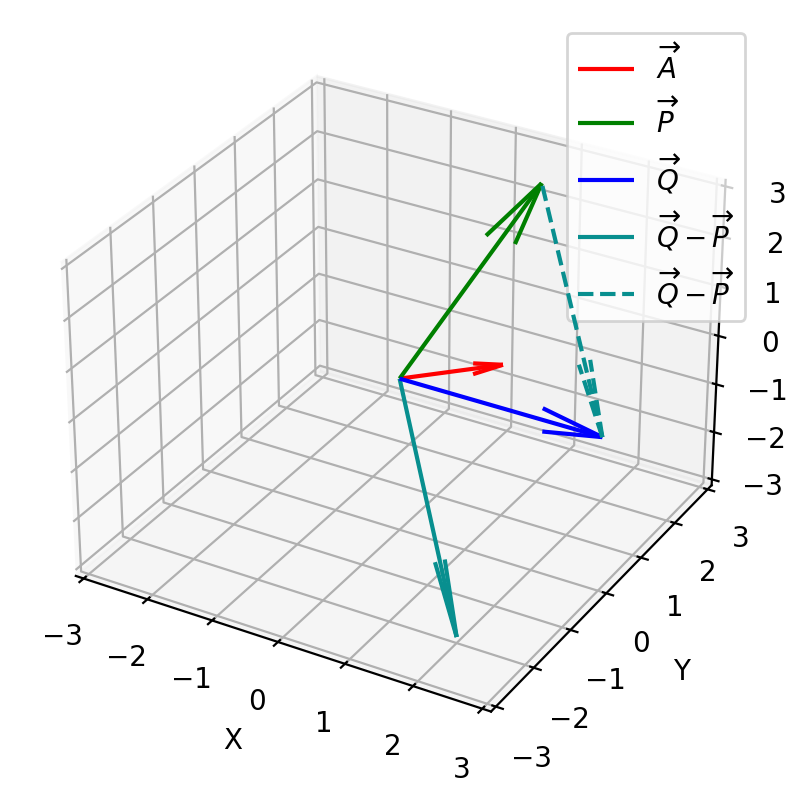
\includegraphics[width=\linewidth]{Q1.png}\label{fig:Q1}
\end{figure}

\section{Question 2}

\subsection{Problem}

Find the shortest distance between point \(P(3, 1, 2)\) and the plane given by
\(x - 2y + z = 5\).

\subsection{Solution}

\[\boldsymbol{d}=|(\vec{P}-\vec{A}) \cdot \widehat{\boldsymbol{n}}|\]

\[
    \vec{P} = \left\langle3, 1, 2\right\rangle
\]

We could substitute in the plane equation to get \(\vec{A}\).

\[
    \vec{A} = \left\langle 0, 0, 5\right\rangle
\]

\[
    \widehat{\boldsymbol{n}} = \frac{\vec{n}}{\left\lvert \vec{n} \right\rvert } = \frac{\left\langle 1, -2, 1\right\rangle}{\sqrt{6}}
\]

\[
    \boldsymbol{d} = \frac{1}{\sqrt{6}}\left\lvert \sum_i {(P_i - A_i)n_i}\right\rvert
    = \frac{\left\lvert 1(3 - 0) + -2(1 - 0) + 1(2 - 5)\right\rvert }{\sqrt{6}}
    = \frac{2}{\sqrt{6}}
\]

\begin{figure}[H]
    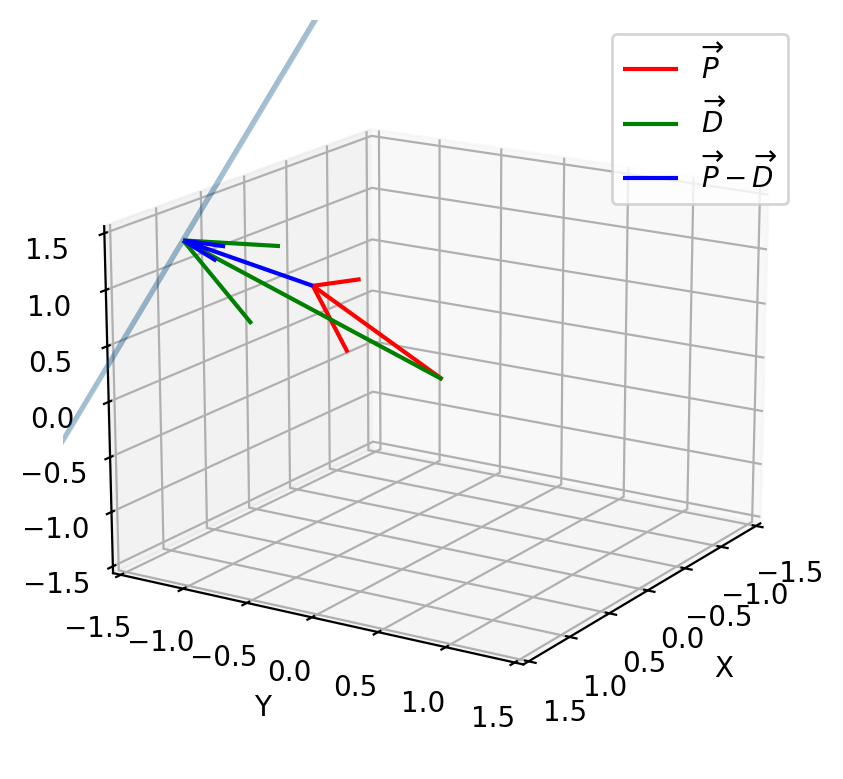
\includegraphics[width=\linewidth]{Q2.png}\label{fig:Q2}
\end{figure}

\section{Question 3}

\subsection{Problem}

Find a unit vector that is orthogonal to the line

\[
    x = 2t - 1, y = -t - 1, z = t + 2
\]

and the vector \(\hat{\dot{\imath}} - \hat{\dot{\jmath}}\).

\subsection{Solution}

From the parametric equations of the line, we can get the direction vector of the line.

\[
    \mu = \left\langle 2, -1, 1\right\rangle
\]

\[
    \mu \times \left\langle 1, -1, 0\right\rangle
    = \left\lvert
    \begin{array}{ccc}
        \hat{\dot{\imath}} & \hat{\dot{\jmath}} & \hat{k} \\
        2 & -1 & 1 \\
        1 & -1 & 0
    \end{array}
    \right\rvert
\]

\[
    = \hat{\dot{\imath}} + \hat{\dot{\jmath}} + -\hat{k}    
\]

\[
    \vec{x} = \pm \left\langle 1, 1, -1\right\rangle
\]

\section{Question 4}

\subsection{Problem}

A line is given by \(\vec{r} = \vec{a} + \lambda \vec{b}\)
where \(\vec{a} = \hat{\dot{\imath}} + 2 \hat{\dot{\jmath}} + 3 \hat{k}\)
and \(\vec{b} = 4 \hat{\dot{\imath}} + 5 \hat{\dot{\jmath}} + 6 \hat{k}\).
Find the coordinates of the point at which the line intersects the plane \(2x + y + 3z = 6\).

\subsection{Solution}

\section{Question 5}

\subsection{Problem}

Starting with the vector quadruple product
\[
    (\vec{A} \times \vec{B}) \times(\vec{C} \times \vec{D})
\]

Show that \(\vec{D}\) can be expressed as a linear combination of \(\vec{A}, \vec{B}, \vec{C}\).

\subsection{Solution}

\bibliographystyle{plain}
\bibliography{references}
\nocite{El-Deeb_PEU-218_Assignments}

\end{document}